$k^2$-tree est une structure de donnés dense conçue à l'origine pour la compression des graphes du web, l'algorithme de base a été proposé par Bisaboa et all dans leur article $k^2$-trees for Compact Web Graph. \citep{brisaboa2009k} Elle a été appliquer ensuite dans d'autres travaux de compression comme les réseaux sociaux \citep{shi2012optimizing}, les rasters \citep{de2013compact} et les bases de donnés RDF \citep{alvarez2017succinct}.\\
%%n oublie pas les réf pour chaque domain d application 
  
En général, l'algorithme peut être appliquer a n'importe quelle matrice binaire. Dans le cadre de notre étude nous nous intéressons seulement à la matrice d'adjacence d'un graphe.
$k^2$-trees exploite les propriétés de la matrice d'adjacence et tire parti des zones vides pour réduire l'espace de stockage et permettre au graphe de tenir en mémoire central. il offre aussi la possibilité de naviguer dans le graphe sans le décompresse, et de répondre aux requêtes de voisinage direct et inverse.

Étant donné une matrice d'adjacence A d'ordre n, $k^2$-trees représente A sous forme d'un arbre de recherche $k^2$-air * de hauteur h = [$log_{k}$ n], chaque nœud contient un seul bit avec deux valeurs possible : 1 pour les nœuds interne et 0 pour les feuilles, sauf le dernier niveau où les feuilles représentent les cases de A et peuvent prendre une valeur 0 ou 1. La racine correspond au premier niveau et prend une valeur 0. chaque nœud interne de l'arbre a exactement $k^2$ fils.  
Avant la construction de l'arbre, il faut s'assurer que n est une puissance de k, dans le cas inverse, l'algorithme étend la matrice en rajoutant des zéros à droite et en bas de la matrice, l'ordre de la matrice deviens donc n'= $k^{log_{k} n}$.\\

Pour construire l'arbre, $k^2$-trees commence par deviser la matrice en $k^{2}$ sous matrice d'ordre n/k, la racine correspond à la matrice complète, chaque sous matrice représente un nœud dans le premier niveau de l'arbre, elle est ajouté comme un fil à la racine suivant un ordre de gauche à droite et de haut en bas. Le nœud est à 1 si la sous matrice qu'il représente contient au moins un 1, et à 0 si elle ne contient que des 0. le processus est répéter de manière récursive sur les sous matrice représentés par des 1. $k^{2}$ sous matrices sont créé a chaque subdivision. L'opération est répéter jusqu'à ce que la subdivision atteins les cases de la matrice qui représenterons les feuilles de l'arbre au dernier niveau. 

La figure \ref{k2-trees-exemples} illustre la représentation $k^2$-trees d'une matrice de taille $10 \times 10$, étendue a une  taille $16 \times 16$ pour un k=2 \citep{brisaboa2015efficient}.

\begin{figure}[H]
\begin{center}
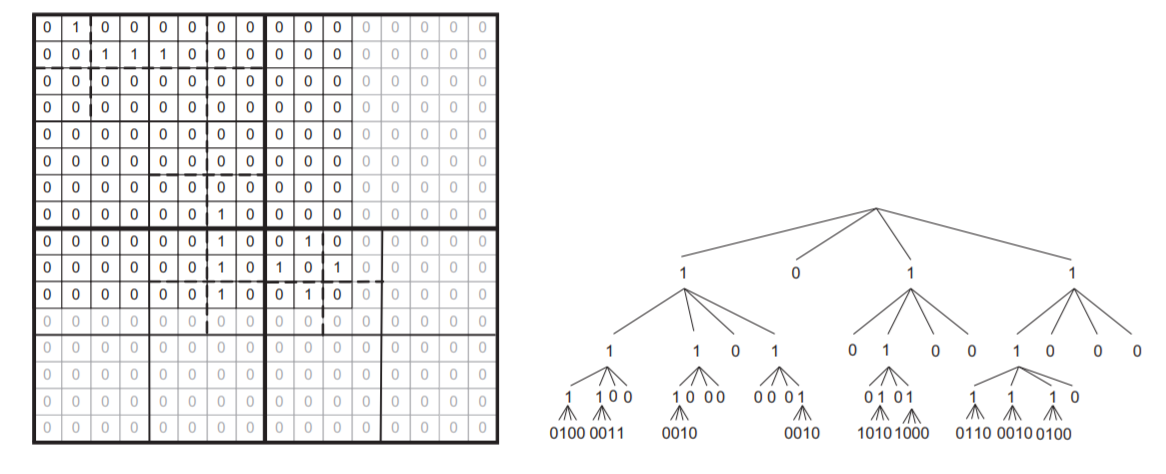
\includegraphics[height=200 pt, width=450 pt]{./ressources/image/k2-trees.png} 
\end{center}
\caption{Exemple de représentation $k^2$-trees d'une matrice d'adjacence d'un graphe}
\label{k2-trees-exemples}
\end{figure}


Pour le stockage de l'arbre, l'algorithme utilise deux tableaux de bits : un tableau T (Tree) contenant tous les nœuds de l'arbre à l'exception du dernier niveau et un tableau L (Leaves) contenant les feuilles du dernier niveau. Les nœuds et les feuilles sont ordonnés selon un parcours en largeur de l'arbre.   
Ci-dessous les deux tableaux T et L de l'exemple précédent (figure \ref{k2-trees-exemples}) : \\
T = 1011 1101 0100 1000 1100 1000 0001 0101 1110\\
L = 0100 0011 0010 0010 1010 1000 0110 0010 0100\\
Dans le pire des cas, l'espace totale pour la description de la structure est $k^2$m($log_{k^2}\frac{n^2}{m}$+ \textit{O}(1)), où n est le nombre de nœuds du graphe et m le nombre de liens. Cependant, pour les graphe du monde réel, l'espace nécessaire pour le stockage est bien meilleur. \\

Dans le même travail \citep{brisaboa2009k}, et dans le but d'obtenir un compromis entre la taille de l'arbre et le temps de parcours , les auteurs ont proposé une hybridation qui consiste a changer la valeur du paramètre k en fonction du niveau de l'arbre en donnant a k une grande valeur au début pour réduire le nombre de niveaux et améliorer ainsi le temps de recherche, et une petite valeur a la fin pour avoir des petites sous matrices et réduire l'espace de stockage.\\
Pour le stockage de l'arbre, un tableau $T_{i}$ est utilisé pour chaque valeur $k_{i}$, le tableau L reste le même.\\

Plusieurs variantes de l'algorithme de base ont été proposés dans la littérature dont le but était soit d'obtenir un meilleur résultat de compression, soit d'appliquer la méthode sur d'autres types de graphes. Nous allons dans ce qui suit présenter les travaux qu'on a put trouver.\\

Dans \citep{shi2012optimizing}, les auteurs proposent deux techniques d'optimisation de l'algorithme : la première consiste à trouver un certain ordre de nœuds qui permet de regrouper les 1 de la matrice d'adjacence dans une seule sous matrice au lieu qu'ils soient dispersés de manière aléatoire. La recherche d'un ordre optimal des nœuds est inenvisageable, avec k=2, le problème peut être réduit à un autre problème (min bisection) qui est NP-difficile, et quand k est dynamique le problème est plus compliqué. Comme solution, les auteurs utilisent DFS avec des heuristiques pour trouver une approximation de l'ordre optimal. Cette optimisation permet de réduire le nombre de nœuds internes et produire ainsi un arbre optimal. la deuxième optimisation est de trouver la valeur de k la plus adéquate pour chaque nœud interne, calculer cette valeur pour chaque nœud peut engendrer un temps de calcul très important. Pour éviter cela, les auteurs affectent la même valeur k pour les nœuds ayant le même parent. 	

Dans \citep{brisaboa2014compact}, les auteurs apportent deux amélioration principales dans le but d'optimiser l'espace et le temps de parcours de l'arbre produit : la première est de construire $k^2$ arbres distincts pour les $k_{0}^{2}$ sous matrices du premier niveau, cella à plusieurs avantages, premièrement, l'espace est réduit étant donné que la taille de chaque arbre est en fonction de $\frac{n^2}{k^2}$,deuxièmement le temps de parcours s'améliore puisque T et L sont plus petits. la deuxième amélioration est la compression de L qui consiste à construire un vocabulaire \textit{V} de tous les sous matrices du dernier niveau sous forme de séquences de bits, les classer par fréquence d'apparition et remplacer leurs occurrence dans L par des pointeurs, cela permet d'éviter la redondance et réduire par suit la taille de la structure. Les pointeur sont représenté par des codes de longueur variable ordonné, le plus petit correspond a la sous matrice la plus fréquente. Néanmoins, cette représentation ne permet  pas un accès direct dans L étant donné qu'une décompression séquentiel est nécessaire pour récupérer une position, pour remédier à ce problème les auteurs utilisent le principe de Directly Addressable Codes (DACs) \citep{brisaboa2013dacs} pour garantir un accès rapide au pointeur et conserver ainsi une navigation efficace.\\
Exemple : Pour la figure \ref{k2-trees-exemples}, le vocabulaire et L sont représentés comme suit :\\
\textit{V}= [0010 0100 0011 1010 1000 0110]\\
L = $c_{1}c_{2}c_{0}c_{0}c_{3}c_{4}c_{5}c_{0}c_{1}$ \\

\subsubsection{d$k^2$-trees}
Dans \citep{brisaboa2012compressed}, les auteurs développent la représentation $k^2$-trees pour les graphes dynamique. Ils proposent une nouvelle structure nommé d$k^2$-trees pour dynamique $k^2$-trees qui offre les même capacités de compression et fonctionnalités de navigation que le cas statique et qui permet également d'avoir des mises à jour sur le graphe. Pour atteindre ces objectifs, d$k^2$-trees remplace la structure statique de $k^2$-trees par une implémentation dynamique. Dans cette nouvelle implémentation, les deux tableaux T et L sont replacé par deux arbre, nommés $T_{tree}$ et $L_{tree}$ respectivement. Les feuilles de $T_{tree}$ et $L_{tree}$ stockent des parties des bitmaps T et L. La taille des feuilles est une valeurs paramétré. Les noeuds interns des deux arbres permettent d'accéder au feuilles et  de les modifier.\\
Chaque nœud interne de $T_tree$ contient 3 éléments : deux compteurs b et o qui contiennent respectivement le nombre de bits et le nombre de uns stocké dans les feuilles descendantes de ce nœud, un pointeur P vers le nœud fils. Les nœuds internes de $L_{trees}$ sont similaires sauf qu'ils ne contiennent que b et P. Avec cette structuration, $T_{tree}$ et $L_{tree}$ permettent l'ajout et la suppression des liens dans le graphe.\\
La figure \ref{dk2-trees} présente une représentation d$k^2$-trees : 

\begin{figure}[H]
\begin{center}
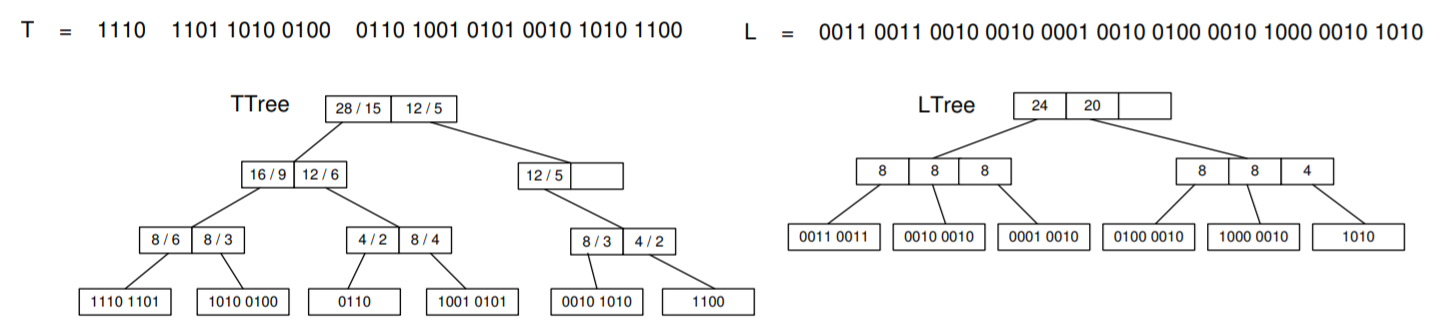
\includegraphics[height=100 pt, width=380 pt]{./ressources/image/dk2-trees.png} 
\end{center}
\caption{Exemple d'une représentation d$k^2$-trees}
\label{dk2-trees}
\end{figure}

\subsubsection{$k^n$-trees}
Dans \citep{de2013compact}, Sandra and al présente $k^n$-trees, une généralisation des $k^2$-trees pour les problème multidimensionnelles. Cette méthodes a plusieurs applications, elle est utilisé pour représenter les bases de donnés multidimensionnels, les rasters et les graphes dynamique. $k^n$-trees repose sur $k^2$-trees pour représenter une matrice à n-dimensions, la matrice est décomposer en $k^n$ sous-matrice de même taille, comme suit : Sur chaque dimension, K-1 hyperplans devise la matrice dans les position i$\frac{n}{K}$,pour $i \in [1, K-1]$. Une fois les dimensions partitionnés, $k^n$ sous-matrice sont induites, elles sont représenter  par des nœuds dans l'arbre comme dans l'algorithme de base. Les structure utilisés pour le stockage sont aussi les même (T et L).\\
En posant n=3, la méthode peut être appliqué sur les graphe dynamique ou temporelles. Ce type de graphes est représenter par une grille à 3 dimension $X \times Y \times T$, où les deux premières dimensions représentent les nœuds de départ et de destination, et la troisième dimension représente le temps. Une telle représentation peut facilement être stocker avec $k^3$-trees.
La figure \ref{kn-trees} présente une représentation $k^3$-trees d'un graphe dynamique :

\begin{figure}[H]
\begin{center}
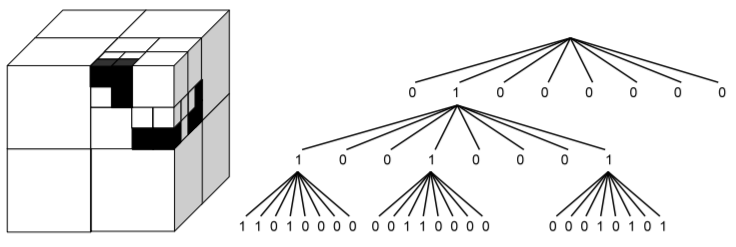
\includegraphics[height=100 pt, width=380 pt]{./ressources/image/kn-trees.png} 
\end{center}
\caption{Exemple d'une représentation $k^3$-trees}
\label{kn-trees}
\end{figure}



\subsubsection{$K^2$-tress1 }
Une autre variante de la méthode a été proposé par \citep{de2014new}. La représentation de base regroupe seulement les zones de zéros, puisque elle a été conçue au début pour les graphe du web qui possèdent une matrice d'adjacence extrêmement creuse. Les auteurs proposent d'étendre cette représentation en regroupant les zones de uns également. L'idée générale est d'arrêter la décomposition de la matrice d'adjacence quand une zone unis est trouvé, à savoir des zéros où des uns. Pour distinguer entre les différents nœuds, une représentation quadtree est utilisée \citep{de1997computational} : une couleur est attribué à chaque nœud, blanc pour une zone de zéro, noir pour une zone de uns et gris pour les nœuds internes e.i. les zones contenant des uns et des zéros. Pour le stockage des nœuds, les auteurs ont proposé quatre encodages présenter par la suite : \\

\textbf{ $k^2$-$trees1^{2-bits-naive}$ :} Dans cet encodage, deux bits sont utilisés pour représenter chaque type de nœud. L'attribution des bits n'est pas arbitraire, le premier bit du poids fort indique si le nœud est un nœud interne (0) ou une feuille (1), le deuxième détermine si les feuilles sont blanches (0) où noires (1). Nous aurons donc : 10 pour les nœuds gris, 01 pour les nœuds noir et 00 pour les nœuds blancs. Notant que les feuilles du dernier niveau sont représenter par un seule bit.
Après le codage, les premier bits de chaque nœud sauf ceux du dernier niveau sont stocker dans T, un autre tableau T' est créer pour sauvegarder les deuxièmes bits, les nœuds du dernier niveau sont stocker dans L.

\textbf{ $k^2$-$trees1^{2-bits}$ :} Le même principe de l'encodage précédant sauf que les nœuds gris sont représenter par un seul bit, toujours à 1, le tableau T' va contenir dans ce cas la couleur des feuilles, cela va réduire la taille de la structure.

\textbf{ $k^2$-$tree1s^{DF}$ :} Cet encodage est similaire à $k^2$-$trees^{2-bits}$, mais il utilise un seul bit pour les nœuds blancs et 2 bits pour les nœuds noirs et gris, compte tenue de la fréquence des nœuds blanc dans les graphe du monde réel par rapport au autres. Nous aurons donc : 0 pour les noeuds blancs, 10 pour les nœuds gris et 11 pour les nœuds noir.

\textbf{ $k^2$-$trees1^{5-bits}$ :} le dernier encodage repose sur la représentation de base, un nœud blanc est représenté par 0, un nœud noir où gris par 1, exactement comme le $k^2$-trees d'origine. Pour identifier un nœud noir (zone de uns), il sera représenté par une combinaison impossible : $k^2$ fils de 0 sont ajouté au nœud noir pour le distinguer.


La figure \ref{k2-trees1-exemple} illustre une représentation $k^2$-tress1 avec les quatre encodage : 


\begin{figure}[H]
\begin{center}
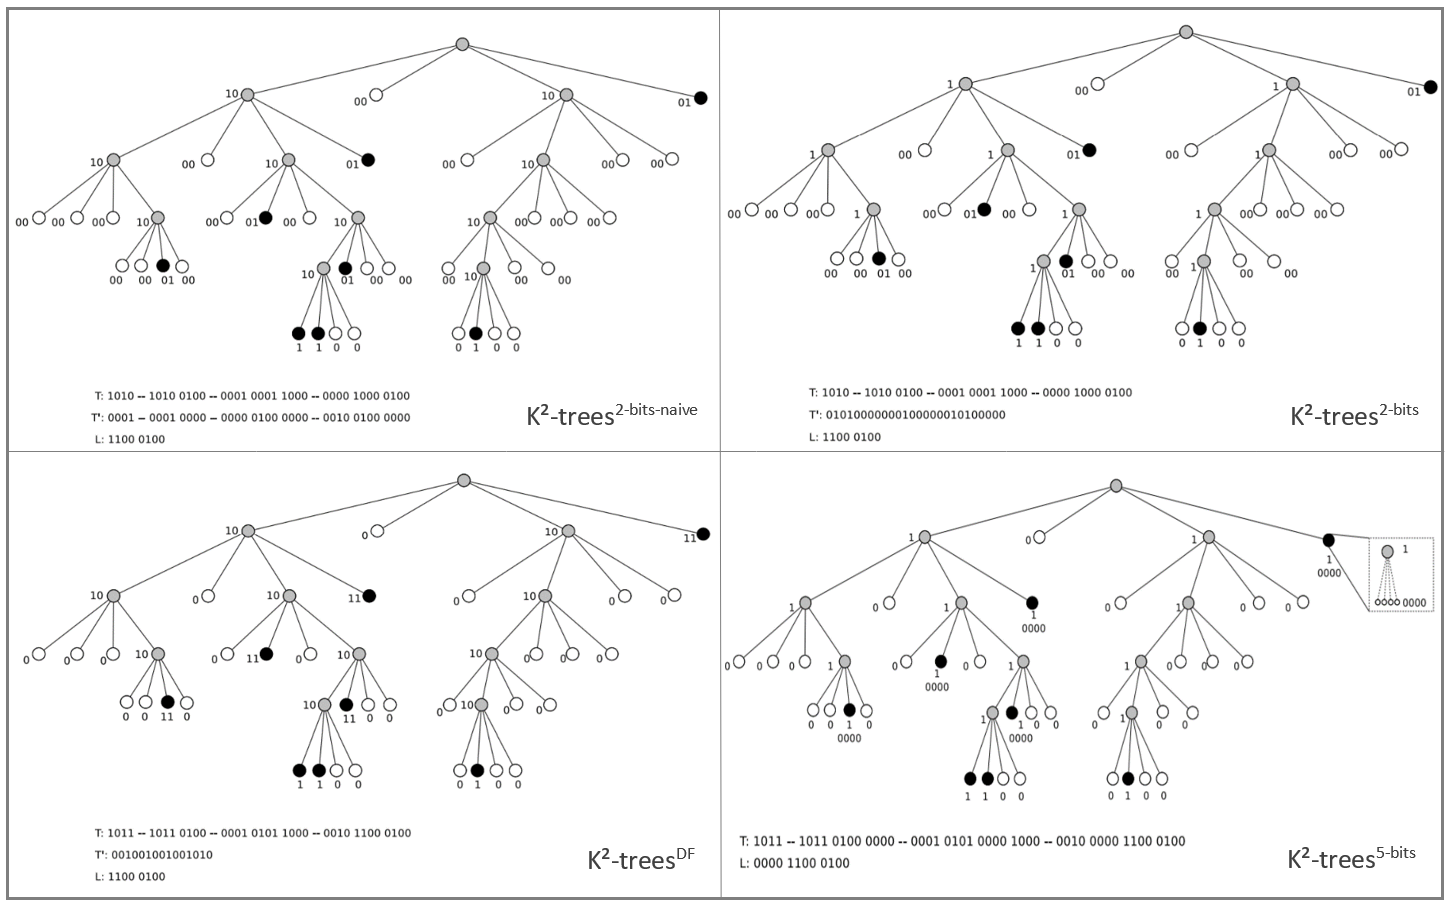
\includegraphics[height=300 pt, width=450 pt]{./ressources/image/k2-trees1.png} 
\end{center}
\caption{Exemple de représentation $k^2$-trees1 d'une matrice d'adjacence d'un graphe}
\label{k2-trees1-exemple}
\end{figure}


\subsubsection{Delta-$K^2$-tress }

Dans \citep{zhang2014delta}, les auteur proposent Delta-$k^2$-trees, une variante qui exploite la propriété de similarité entre les nœuds voisins du graphe pour réduire le nombre de uns dans la matrice d'adjacence. Notons par \textit{Matrix} la matrice d'adjacence, Delta-$k^2$-trees construit une nouvelle matrice appelé \textit{Delta-matrix}, une ligne \textit{i} de \textit{Delta-matrix} va contenir la différence entre les deux lignes \textit{Matrix}[i] et  \textit{Matrix}[i-1] si cela décroit le nombre de uns sinon elle sera égale à \textit{Matrix}[i]. e.i. : \\

$\left\{
\begin{array}{llcl}
Delta-matrix[i] & := matrix[i] & si & count1s(matrix[i]) < countDif(matrice[i],matrix[i-1]) \\
Delta-matrix[i] & := matrix[i] \bigoplus matrix[i-1] &  sinon
\end{array}
\right.$\\

Où count1s compte le nombre de 1 dans une ligne, countDif compte le nombre de bits différent entre deux ligne et $\bigoplus$ représente le ou exclusif.\\
Pour déterminer si une ligne est identique a celle de la matrice d'adjacence, un tableau D est utilisé : Si D[i]=1 la ligne est identique ,sinon elle est une ligne de différence.\\
La matrice \textit{Delta-matrix} contient moins de uns que la matrice d'adjacence, d'où elle est plus creuse, ce qui permet de réduire la taille de la structure et avoir un meilleur taux de compression. Cependant le temps de parcours est plus grand car pour accéder a certains lignes (lignes de différence), le graphe doit être décompresser et la matrice d'adjacence reconstituer\\

La figure \ref{k2-trees-delta} présente un exemple de la représentation Delta-$k^2$-trees


\begin{figure}[H]
\begin{center}
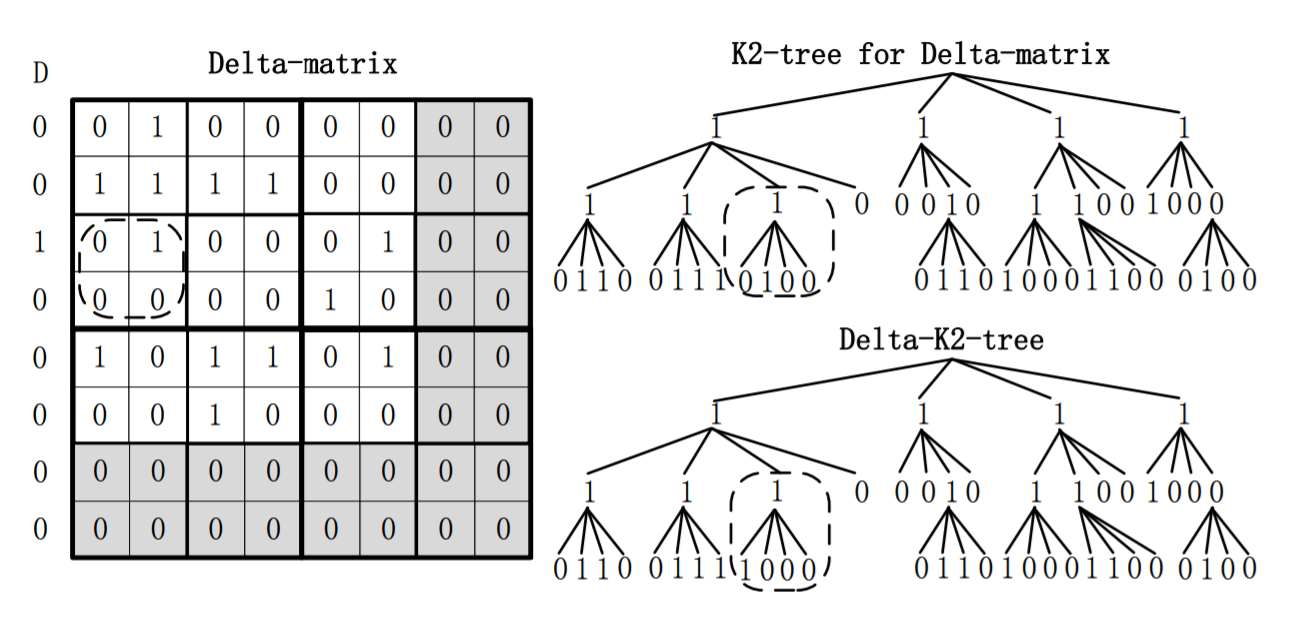
\includegraphics[height=150 pt, width=380 pt]{./ressources/image/k2-trees-delta.png} 
\end{center}
\caption{Exemple de représentation Delta-$k^2$-trees d'une matrice d'adjacence d'un graphe}
\label{k2-trees-delta}
\end{figure}

\subsubsection{$K^2$-treaps }
$K^2$-treaps est une autre variante de $k^2$-trees,elle a été proposé dans \citep{brisaboa2014k}. Cette variante combine les $k^2$-trees avec une autre structure de donnés appelé treaps \citep{aragon1989randomized}, les auteurs applique cette méthode sur des grilles multidimensionnels comme OLAP pour pouvoir les stocker et répondre efficacement aux requêtes top-K \citep{badr2013traitement}. La méthode peut être également appliqué sur les graphe pondéré, où chaque case de la matrice d'adjacence du graphe comporte le poids de l'arrêt qu'elle représente au lieu d'un 1.
Une décomposition récursive en $k^2$ sous-matrice est appliqué sur la matrice d'adjacence et un arbre $k^2$-air est construit comme dans l'algorithme de base, comme suit : la racine de l'arbre va contenir les coordonnés de la cellule avec le plus grands poids de la matrice, ainsi que sa valeur. La cellule qui vient d'être ajouté à l'arbre est ensuite supprimé de la matrice. Si plusieurs cellules ont la même valeurs maximales, l'une d'elles est choisis au hasard. Ce processus est répété récursivement sur chaque sous matrice en choisissant la cellule la plus lourde qu'elle contient pour la représenter dans l'arbre avec ses coordonnés et sa valeurs, et supprimer la cellule choisis au final. La procédure contenue sur chaque branche de l'arbre jusqu'à ce qu'on tombe sur les cellules de la matrice d'origine où sur une sous matrice complètement vide.\\
La figure \ref{k2-treaps} suivante illustre le représentation $k^2$-treaps d'un graphe pondéré \citep{badr2013traitement} :

\begin{figure}[H]
\begin{center}
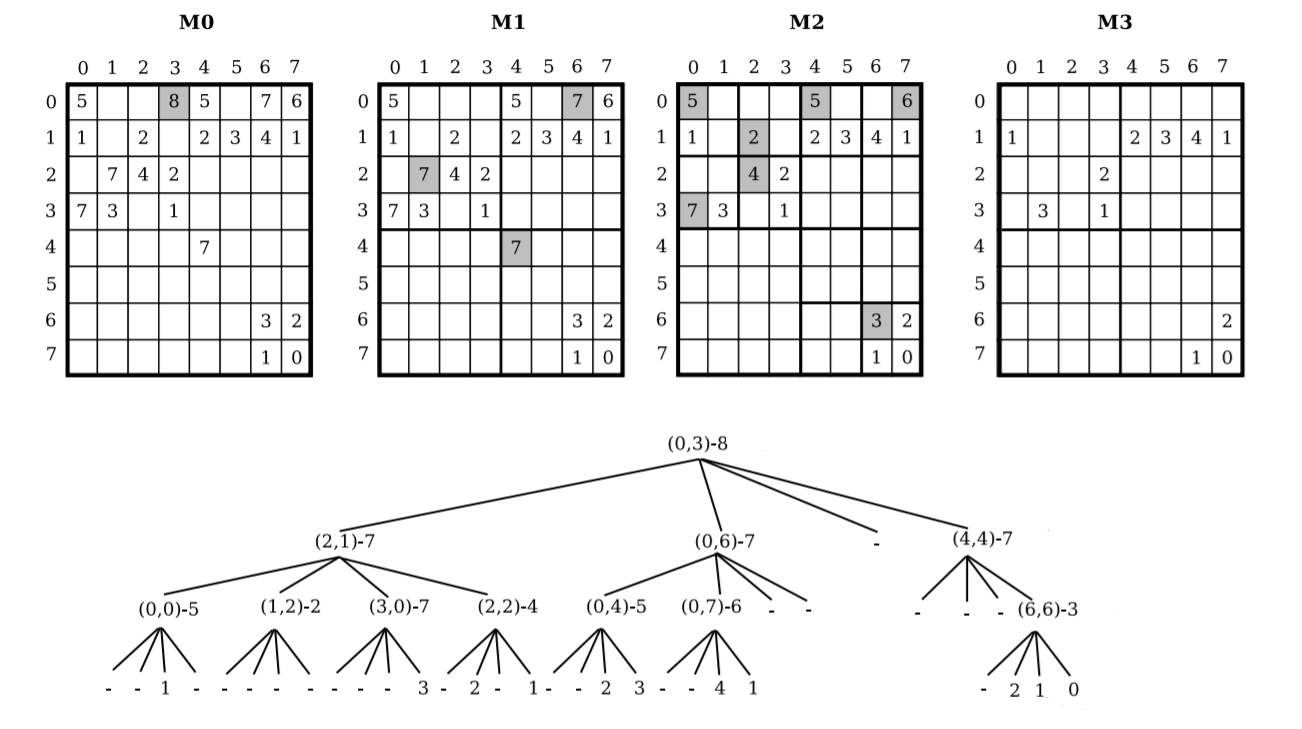
\includegraphics[height=200 pt, width=380 pt]{./ressources/image/k2-treaps.png} 
\end{center}
\caption{Exemple de représentation $k^2$-treaps d'une matrice d'adjacence d'un graphe pondéré}
\label{k2-treaps}
\end{figure}

\textbf{Structure de donnés :} Pour avoir une bonne compression, $k^2$-treaps effectue des transformation sur les donnés stockés . La première transformation consiste a changer les coordonné  représenté dans l'arbre en des coordonné relative par rapport a la sous matrice actuelle, la deuxième est de remplacer chaque poids dans l'arbre par la différence entre sa valeur et celle de son parent.\\
Trois structures de donnés sont utilisés pour sauvegarder les coordonnés et les valeurs des cellules ainsi que la topologie de l'arbre. Chaque structure est détaillé dans ce qui suit :
\begin{itemize}
\item \textit{Listes de coordonnés locales :} la séquence de coordonnés de chaque niveau \textit{l} de l'arbre est stocké dans une liste \textit{coord}[\textit{l}].
\item \textit{liste des valeurs : } Le parcours de l'arbre se fait en largeur, la séquence de valeurs récupéré est stocké dans une liste nommé \textit{values}. Un tableau nommé \textit{first} est utilisé pour sauvegarder la position de commencement de chaque niveau dans \textit{values}.
\item \textit{L'arbre :} la structure de l'arbre $k^2$-treaps est sauvegarder avec un arbre $k^2$-trees, les nœuds contenant des valeur dans $k^2$-treaps sont représenter par des uns, les nœuds vides par des zéros. Pour le stockage de l'arbre, un seul tableau T est utilisé. 
\end{itemize}

La figure \ref{k2-treaps-structure} représente les structures de donnés utilisés pour le stockage de l'arbre de la figure \ref{k2-treaps} précédente \citep{badr2013traitement} :

\begin{figure}[H]
\begin{center}
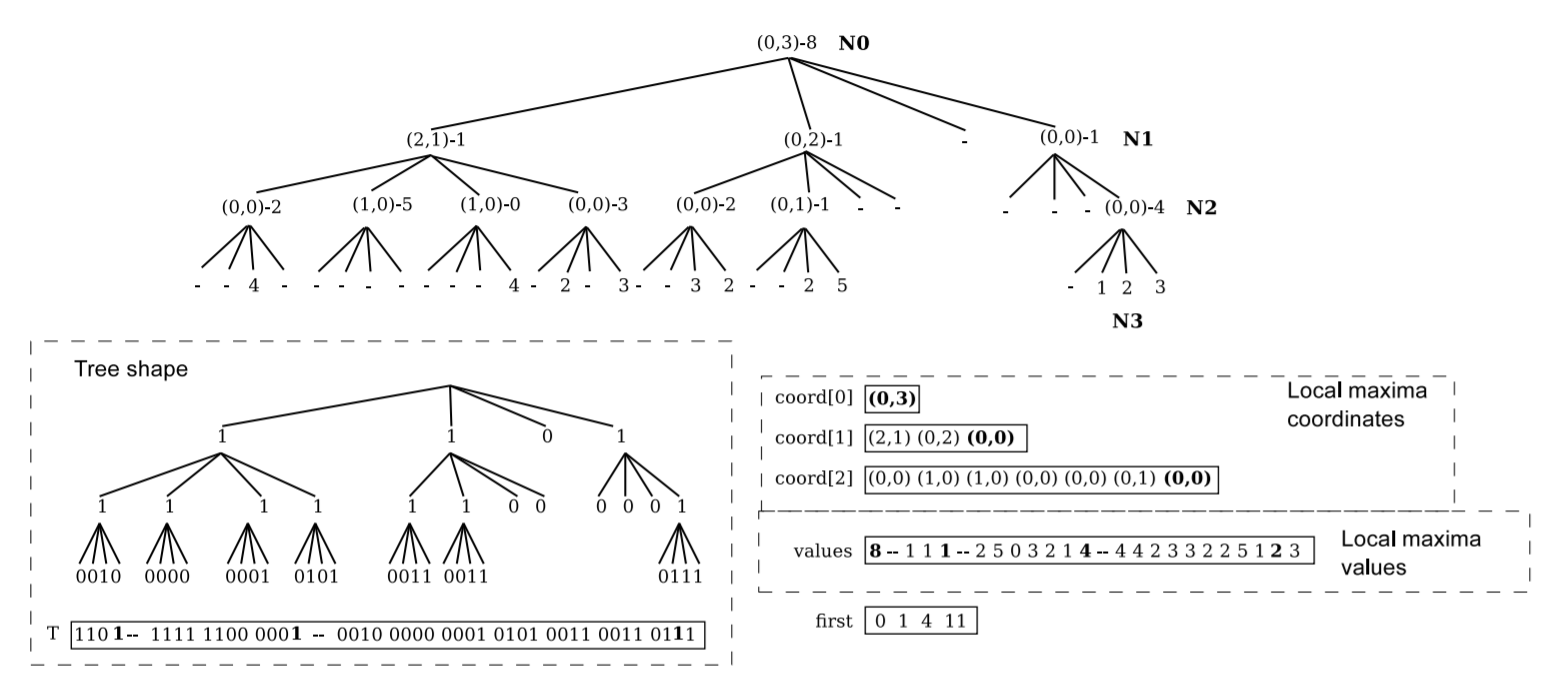
\includegraphics[height=200 pt, width=380 pt]{./ressources/image/k2-treaps-structure.png} 
\end{center}
\caption{Structures de donnés pour une représentation $k^2$-treaps d'une matrice}
\label{k2-treaps-structure}
\end{figure}

\subsubsection{I$k^2$-trees}
Une autre représentation a été proposé par \citep{garcia2014interleaved}, intitulé I$k^2$-trees pour Interleaved $k^2$-trees, Elle est appliqué sur les bases de donnés RDF ainsi que sur les graphe dynamique. Les auteurs proposent cette méthodes pour les relations ternaires, Une relation ternaire est définit par un triplet T=\{ $x_i$,$y_j$,$t_k$ \} $\subseteq$ $ X \times Y \times T$, I$k^2$-trees transforme cette relation en |Z| relation binaire . Dans les graphe dynamique, les deux premières dimension correspondent aux nœuds sources et destination et la troisième dimension reflète le temps. Le graphe est donc définit par |T| matrices d'adjacence prise à des instants $t_k$ différents. I$k^2$-trees représente les matrices simultanément, chaque matrice est représenté par un arbre $k^2$-trees, les arbre sont par la suit regroupé dans un seul arbre. Chaque nœuds de l'arbre obtenue représente une sous-matrice comme dans l'algorithme de base, sauf qu'au lieu d'utiliser un seule bit, I$k^2$-trees utilise 1 à |T| bits pour représenter le nœud. Le nœud racine contient |T| bits. Le nombre de bits de chaque fils est donné par le nombre de uns de son parent. l'arbre final est stocké comme dans l'original $k^2$-trees avec deux tableau : T et L.\\
La figure \ref{Ik2-trees} est un exemple de I$k^2$-trees appliqué sur un graphe dynamique représenté sur trois instants

\begin{figure}[H]
\begin{center}
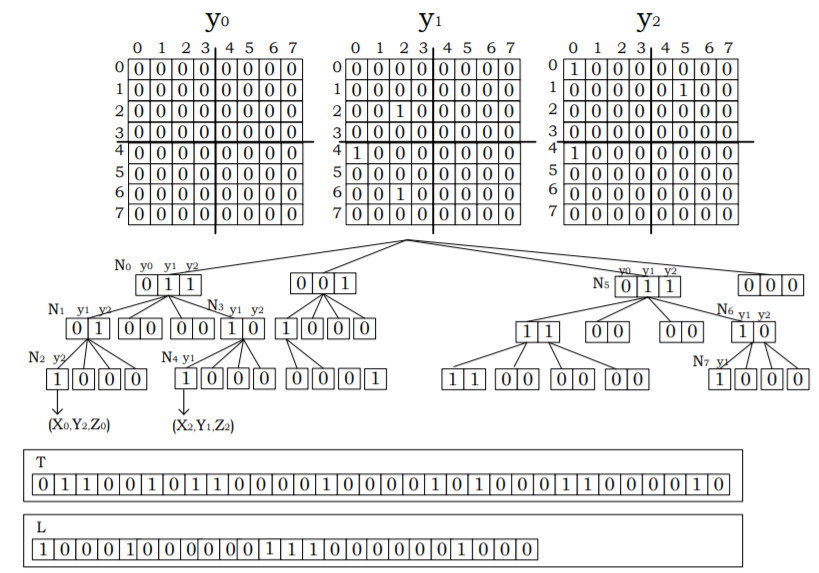
\includegraphics[height=200 pt, width=380 pt]{./ressources/image/Ik2-trees.png} 
\end{center}
\caption{Exemple d'une représentation I$k^2$-trees}
\label{Ik2-trees}
\end{figure}

\subsubsection{diff I$k^2$-trees}
Une variante de I$k^2$-trees appelé Differential I$k^2$
-tree a été étudié dans \citep{alvarez2017succinct}, son but est d'améliorer le taux de compression en représentant uniquement les changements survenue sur le graphe à un instant $t_i$ au lieu d'une instance complète : A l'instant $t_0$, une capture complète du graphe (matrice d'adjacence) est stocké. A l 'instant $t_k$, pour k>0, seuls les arrêtes qui change de valeurs entre $t_{k-1}$ et $t_k$ sont stockés. Les matrices sont représenter a la fin de la même manière que I$k^2$-trees. La limite de cette représentation est que la structure doit être décompresser lors d'une requêtes. \\
La figure \ref{Ik2-trees-diff} montre un exemple d'une représentation diff I$k^2$-trees.

\begin{figure}[H]
\begin{center}
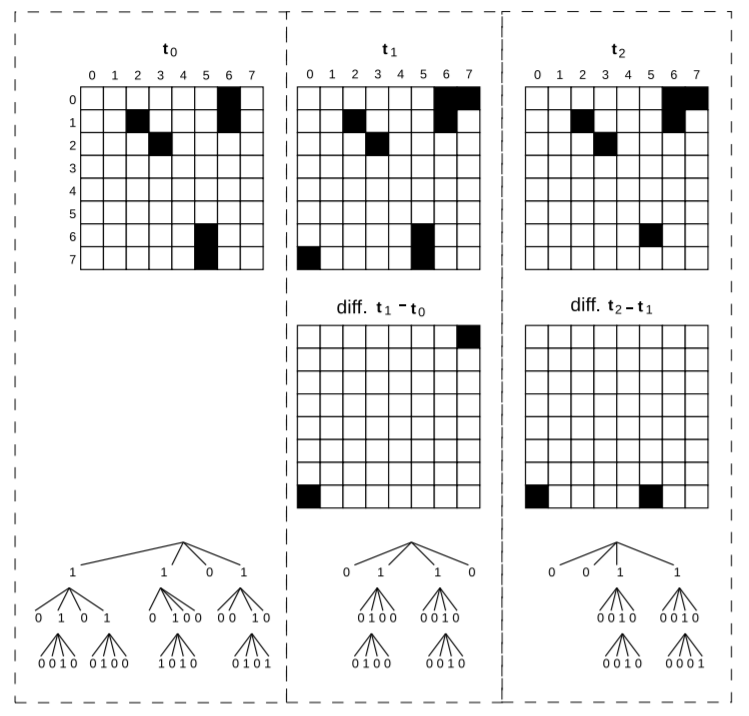
\includegraphics[height=200 pt, width=380 pt]{./ressources/image/Ik2-trees-diff.png} 
\end{center}
\caption{Exemple d'une représentation diff I$k^2$-trees}
\label{Ik2-trees-diff}
\end{figure}

\subsubsection{Att $K^2$-trees }
Dans \citep{alvarez2018compact}, les auteurs étendent la représentation $k^2$-trees pour les bases de donnés orienté graphe. Ces graphes sont étiquetés, attribués, orientés et ont des arrêtes multiples. Ils présentent le graphe sous forme d'une nouvelle structure intitulé Att $k^2$-trees pour Attributed $k^2$-trees.\\
La figure \ref{k2-trees-att-graphe} montre un exemple de graphe pris en compte par Att $K^2$-trees

\begin{figure}[H]
\begin{center}
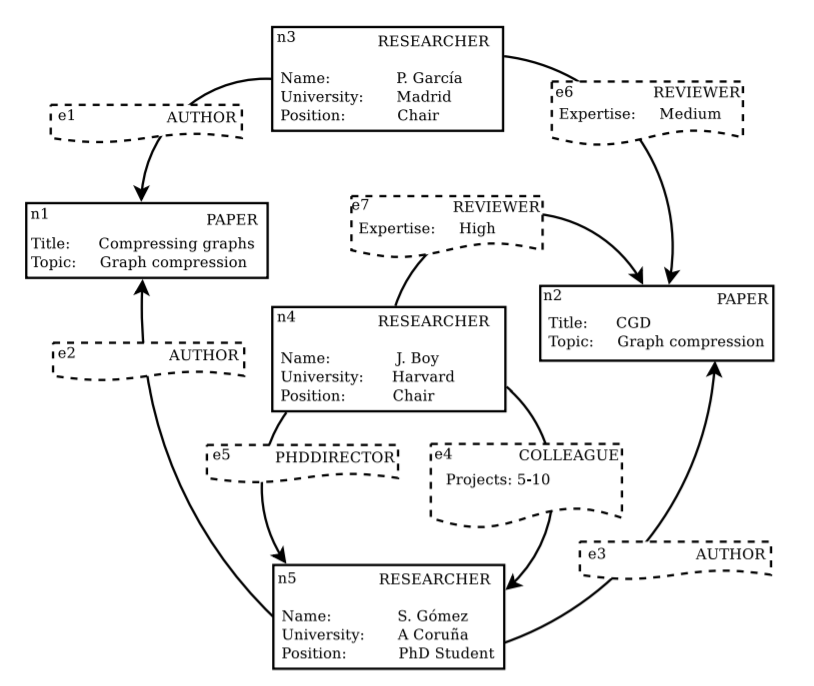
\includegraphics[height=200 pt, width=280 pt]{./ressources/image/k2-trees-att-graphe.png} 
\end{center}
\caption{Exemple d'un graphe étiqueté, attribué, orienté et multiple}
\label{k2-trees-att-graphe}
\end{figure}

\textbf{Structures de donnés :} La représentation obtenue par la compression est composer d'un ensemble d'arbres $k^2$-trees et d'autres structures supplémentaires. Le graphe est représenter par trois composants : un schéma de donnés, les donnés incluse dans les nœuds et les liens et finalement la relation entre les éléments du graphe. Chaque composant est présentés dans ce qui suit :
\begin{itemize}
\item \textit{Schéma : } Ce composant gère les étiquette et les attribues de chaque type d'éléments, il joue le rôle d'un indexe dans la représentation. Il est composé de :
\begin{description}
\item[Un schéma de nœuds :] représenter par un tableau qui contient les étiquètes des nœuds du graphe ordonné lexicographiquement. Un identifiant est attribué a chaque nœud du graphe selon l'ordre du tableau, les \textit{$m_1$} possédant la première étiqueté du tableau vont avoir des identifiant de 1 à \textit{$m_1$}, les \textit{$m_2$} nœuds avec la deuxième étiquette du tableau vont avoir des identifiants de \textit{$m_1$}+1 à \textit{$m_1$}+\textit{$m_2$} et ainsi de suit. chaque entrée du tableau va stocké  le plus grand identifiant portant son étiquette, cela permet de trouver l'étiquette d'un nœud a travers son identifiant.
\item[Un schéma d'arrêtés :] Comme dans le cas des nœuds, un tableau est utilisé pour stocker les étiquette des arrêtes avec le même principe.  
\end{description}
Le schéma est le point de départ de la représentation, il permet d'obtenir l'étiquette d'un nœud ou d'une arrêt, et d'accéder a ses attributs.
\item \textit{Donnés :} Ce composant contient tous les valeurs que peut prendre un attribut dans le graphe. Un attribut peut être représenter de deux façons différentes selon sa fréquence d'apparition, on distingue donc deux type d'attributs :
\begin{description}
\item[Attributs rares :] Ce sont les attributs qui prennent généralement des valeurs différentes a chaque apparition, ils sont stocker dans des listes et indexer avec l'identifiant de l'élément.
\item[Attributs fréquents :] Ce type d'attributs est sauvegarder dans deux matrices, une pour les attributs des nœuds et l'autre pour les attributs des liens. les matrices sont stocker sous forme d'arbres $k^2$-trees.
\end{description}
La figure \ref{k2-trees-att-schema} illustre les deux composants schéma et donnés de la représentation Att$k^2$-trees  de la figure \ref{k2-trees-att-graphe} précédente
\begin{figure}[H]
\begin{center}
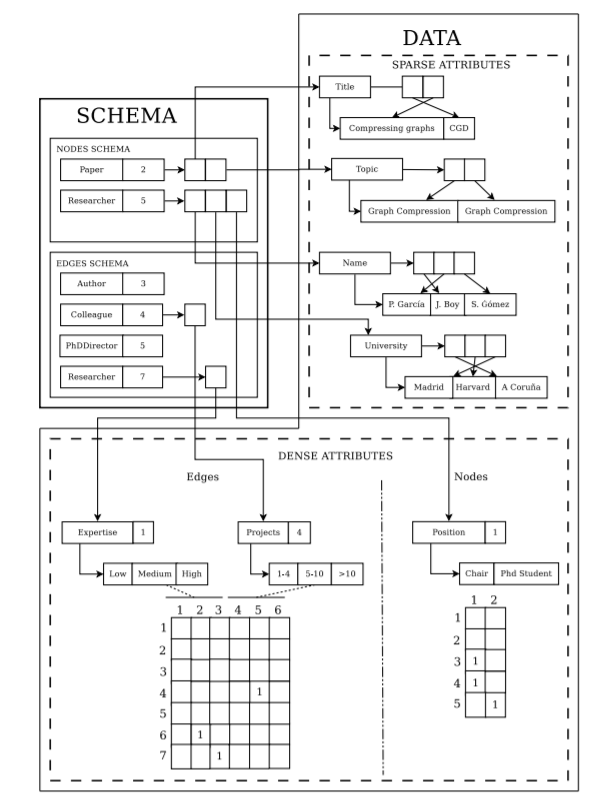
\includegraphics[height=200 pt, width=280 pt]{./ressources/image/k2-trees-att-schema.png} 
\end{center}
\caption{Exemple d'un schéma et donnés de la représentation Att$k^2$-trees}
\label{k2-trees-att-schema}
\end{figure}


\item \textit{Relations :} C'est le dernier composant de Att$k^2$-trees, il stocke les relations entre les nœuds et les arrêtes du graphe en utilisant un arbre $k^2$-trees et d'autres structures pour sauvegarder les identifiants des arrêts ainsi que les arrêtes multiples. Les structures supplémentaires sont les suivants :
\begin{description}
\item[Multi :] Un tableau qui indique si l'arrête est multiple où non.
\item[Firt :] Un Tableau qui donne l'identifiant de l'arrêt, où de celui de la première dans le cas d'une arrête multiple.
\item[Next :] Un tableau qui contient les identifient des arrêtes multiples restantes.
\end{description}
La figure \ref{k2-trees-att-relation} donne la représentation Att$k^2$-trees des relations du graphe de la figure \ref{k2-trees-att-graphe} :
\begin{figure}[H]
\begin{center}
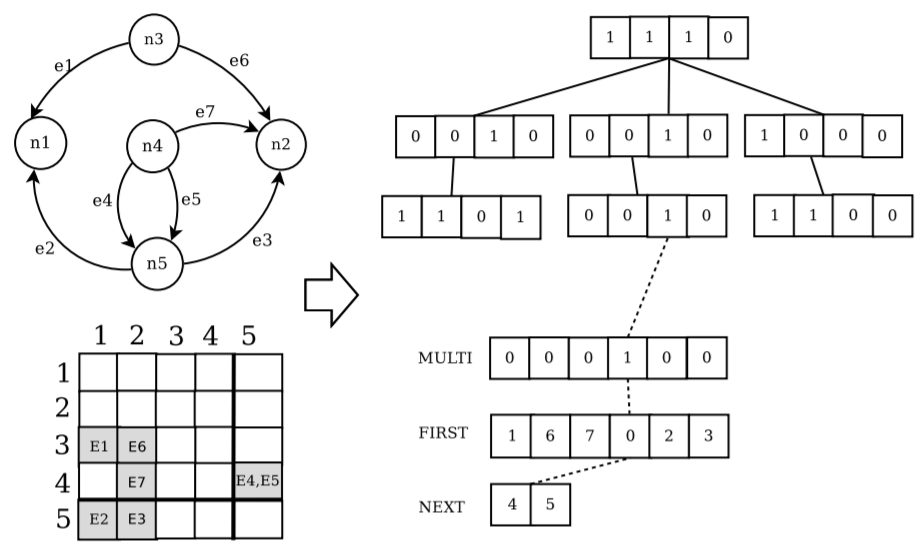
\includegraphics[height=200 pt, width=280 pt]{./ressources/image/k2-trees-att-relation.png} 
\end{center}
\caption{représentation des relations dans Att$k^2$-trees}
\label{k2-trees-att-relation}
\end{figure} 
\end{itemize}

\subsubsection{dynAtt$k^2$-trees }
Dans le même article \citep{alvarez2018compact}, les auteurs étendent Att$k^2$-trees pour les graphes dynamiques, il proposent une nouvelle variante appelé dynAtt$k^2$-trees qui supporte le changement dans les attributs et les liens du graphe. Comme Att$k^2$-trees, dynAtt$k^2$-trees représente le graphe avec trois composants : Schémas, donnés et relations. Les composants sont semblables a ceux de Att$k^2$-trees mais avec certaines amélioration vue la nature dynamique du graphe.\\
\textbf{Structure de donnés : } 
\begin{itemize}
\item \textit{Schéma :}  En ce qui concerne les nœuds, leurs étiquettes sont stockés dans une liste dynamique ordonné lexicographiquement. En outre, une séquence dynamique est utilisé pour sauvegarder le type de chaque nœud, elle est stocké ensuite sous forme d'un arbre d'ondelettes \citep{grossi2003high}. Le même principe est appliqué sur les arrêtes. 
\item \textit{Données :} Les attributs rares sont stockés dans des listes dynamiques, quant aux attributs fréquents, ils sont sauvegardé avec des arbres d$k^2$-trees (un arbre pour chaque attribut).
\item \textit{Relations :} Le stockage des relations se fait à l'aide d'un d$k^2$-trees et des tableaux dynamiques pour stockés les identifiants des arrêtes et les arrêtes multiples.
\end{itemize}




























